
\begin{figure}[b]
    \centering
    \begin{minipage}[t]{.58\textwidth}\vspace{0pt}
    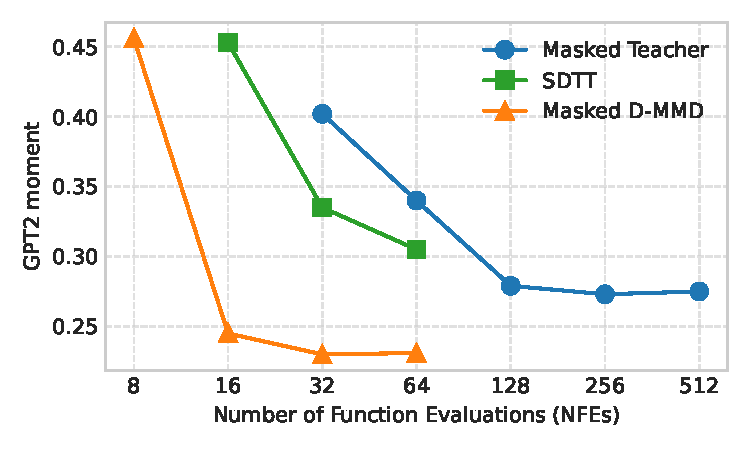
\includegraphics[width=0.99\linewidth]{figures/overview.pdf}
    \end{minipage}
    \begin{minipage}[t]{.38\textwidth}\vspace{.8cm}
    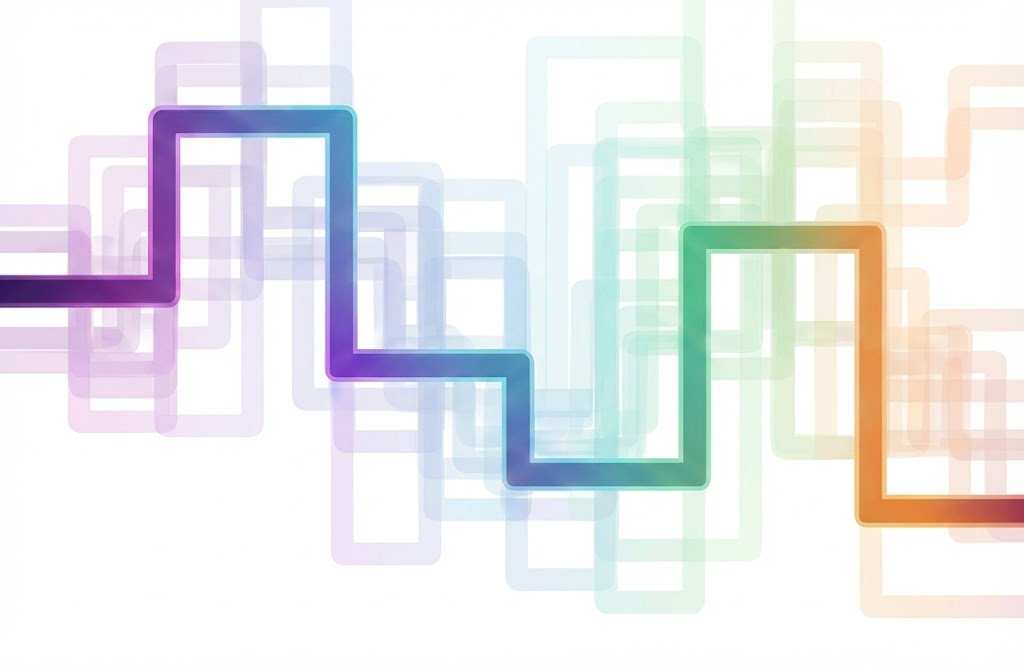
\includegraphics[width=0.99\linewidth]{figures/unnamed-3.jpg}
    \end{minipage}
    \caption{D-MMD text generators match or outperform their teacher using fewer function evaluations.}
    \label{fig:overview}
\end{figure}


\section{Introduction}
Sampling from Discrete Diffusion Models requires many sampling steps. The probability of clean data given noisy data is modeled in a \textit{factorized} manner. I.e., each token is modeled independently conditioned on the previously generated tokens.
As a result, errors from this assumed independence accumulate during the sampling iterations.

Discrete diffusion models perform forward passes on a block of tokens that they currently operate on. Whereas typical causal LLMs have under-utilization problems because they operate on single tokens, diffusion LLMs generally have high accelerator utilization. However, these models tend to need many iterations to converge to a reasonable generation, leading to high computing costs and strictly higher FLOPs. The fewer iterations one takes, the lower the cost.

In this paper we leverage insights from continuous diffusion to distill discrete diffusion models.
Our paper generalizes the formulation of Moment Matching Distillation (MMD) \citep{salimans2024multistep} so that it can be used in more general settings. As our main focus is to distill discrete diffusion processes, we call this new algorithm \emph{Discrete-MMD} (D-MMD).
We show that one can distill few-step generators using D-MMD with sample quality surpassing their teachers on both text and image generation (see \autoref{fig:overview}).
%tasks (see \autoref{fig:overview}).

\lstset{
    literate={“}{{``}}1
           {’}{{'}}1
           {”}{{''}}1,
    breaklines=true,
}
